\documentclass{article}

\usepackage{ctex}
\usepackage{fontspec}
\usepackage{geometry}
\usepackage{fancyhdr}
\usepackage{xcolor}
\usepackage{dashrule}
\usepackage{setspace}
\usepackage{tikz}

\geometry{a4paper, left=2.5cm, right=2.5cm, top=2.5cm, bottom=1.25cm}

\setmainfont{Times New Roman}

\setCJKmainfont[AutoFakeBold]{SimSun.ttc}

\newCJKfontfamily\hwzs{STZhongs.ttf}[AutoFakeBold]
\newfontfamily\hwzseng{STZhongs.ttf}[AutoFakeBold]

\newCJKfontfamily\hwxk{STXingka.ttf}[AutoFakeBold]

% 这里可以自定义课程编号、课程名称、任课教师等信息
\newcommand{\classNumber}{B00000000-00} % 课程编号
\newcommand{\className}{摸鱼大讲堂} % 课程名称
\newcommand{\teacherName}{张三} % 任课教师

% 这里可以自定义页眉的内容
\newcommand{\yearOfTerm}{2024--2025} % 学年开始和结束年份, 请确保中间有两个短横线
\newcommand{\semester}{秋季} % 学期: 秋季/春季
\newcommand{\partTwo}{期末考试} % 页眉第二段内容
\newcommand{\partThree}{本科生试题专用纸} % 页眉第三段内容
%%%%%%%%%%%%%%%%%%%%%%%%%%%%%%%%%%%%%%%%%%%%%%%%%%%%

\pagestyle{fancy}
\fancyhf{}
\fancyhead[C]{\zihao{5} \heiti \yearOfTerm{}学年\semester{}学期 \quad \partTwo{} \quad \partThree{}}
\fancyfoot[C]{\thepage}

\begin{document}

\begin{minipage}[t]{0.4\textwidth}
    \vspace{-0.7cm}
    \begin{center}
        {

        {\zihao{-1} \hwxk 中国科学院大学}

        \vspace{10pt}

        {\zihao{4} \textbf{试 \ 题 \ 专 \ 用 \ 纸}}}
    \end{center}
\end{minipage}
\hspace{3em}
\begin{minipage}[t]{0.4\textwidth}
    \vspace{-0.7cm}
    \fontsize{12.045pt}{14.46pt} \hwzs
    课程编号:{\hwzseng \classNumber}

    \vspace{0.3em}

    课程名称:\className
    \vspace{0.3em}

    任课教师:\teacherName
    \vspace{0.3em}

\end{minipage}

\begin{center}
    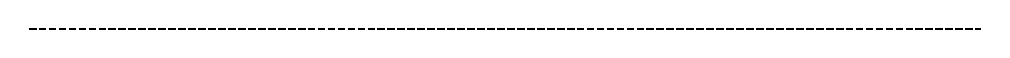
\begin{tikzpicture}
        \draw[dash pattern = on 2.8 pt off 0.8 pt, thick] (0, 0) -- (\linewidth - 1 pt, 0);
    \end{tikzpicture}
\end{center}

\vspace{-0.4cm}

{\hwzs\fontsize{10.53937pt}{10.53937pt}
注意事项:

% 请在下方直接修改 "注意事项" 的内容
% \underline{某些字} 用于给 "某些字" 添加下划线
1. 考核方式:\underline{课程论文+平时成绩}

2. 请在规定时间内将本试卷和答题纸一并交回

}

\vspace{-0.3cm}
\noindent
\rule{\linewidth}{1pt}

\end{document}

